%%%%%%%%%%%%%%%%%%%%%%%%%%%%%%%%%%%%%%%%%%%%%%%%%%%%%%%%%%%%%%%%%%%%%%%%%%%%%%%
%
% witseiepaper-2005.tex
%
%                       Ken Nixon (12 October 2005)
%
%                       Sample Paper for ELEN417/455 2005
%
%%%%%%%%%%%%%%%%%%%%%%%%%%%%%%%%%%%%%%%%%%%%%%%%%%%%%%%%%%%%%%%%%%%%%%%%%%%%%%%%

\documentclass[10pt,twocolumn]{witseiepaper}

%
% All KJN's macros and goodies (some shameless borrowing from SPL)
\usepackage{KJN}

%
% PDF Info
%
\ifpdf
\pdfinfo{
/Title (INSTRUCTIONS AND STYLE GUIDELINES FOR THE PREPARATION OF FINAL YEAR LABORATORY PROJECT PAPERS : 2005 VERSION)
/Author (Ken J Nixon)
/CreationDate (D:200309251200)
/ModDate (D:200510121530)
/Subject (ELEN417/455 Paper Format, 2005)
/Keywords (ELEN417, ELEN455, paper, instructions, style guidelines, laboratory project)
}
\fi

%%%%%%%%%%%%%%%%%%%%%%%%%%%%%%%%%%%%%%%%%%%%%%%%%%%%%%%%%%%%%%%%%%%%%%%%%%%%%%%
\begin{document}


\title{DESIGN AND IMPLEMENTATION OF A HEARTBEAT SEGMENTATION AND CLASSIFICATION MODEL..??}

\author{Boikanyo Radiokana (1386807) \\ Elias Sepuru (1427726)
\thanks{School of Electrical \& Information Engineering, University of the
Witwatersrand, Private Bag 3, 2050, Johannesburg, South Africa}
}


%%%%%%%%%%%%%%%%%%%%%%%%%%%%%%%%%%%%%%%%%%%%%%%%%%%%%%%%%%%%%%%%%%%%%%%%%%%%%%%
%
\abstract{The purpose of this document is to provide an easy-to-use
template/style sheet to enable authors to prepare papers in the correct format
and style for the final year laboratory project. This document may be
downloaded from the School of Electrical and Information Engineering web site
and can be used as a template. To ensure conformity of appearance it is
essential that these instructions are followed. The abstract should be limited
to 50-200 words, which should concisely summarise the paper.}

\keywords{Four to six key words in alphabetical order, separated by commas.}


\maketitle
\thispagestyle{empty}\pagestyle{empty}


%%%%%%%%%%%%%%%%%%%%%%%%%%%%%%%%%%%%%%%%%%%%%%%%%%%%%%%%%%%%%%%%%%%%%%%%%%%%%%%
%
\section{INTRODUCTION}

\section{BACKGROUND}

%%%%%%%%%%%%%%%%%%%%%%%%%%%%%%%%%%%%%%%%%%%%%%%%%%%%%%%%%%%%%%%%%%%%%%%%%%%%%%%
%
\subsection{Project Specifications and Requirements}
\label{PSR}
The aim of this project is to create a first level screening to detect signs of heart diseases in individuals. This will be carried out by using audio data sets from two sources, the iStethoscope Pro iPhone app labelled Dataset A and a digital stethoscope labelled Dataset B. The audio data was recorded by the general public and clinical healthcare practitioners respectively \cite{pascal}. Both data sets A and B each have different categories which all contain various background noises. The audio files vary in length from 1 to 30 seconds as a means of reducing excessive noise \cite{pascal}. Dataset A is said to consist of the the following categories, namely; Normal, Murmur, Extra Heart Sound and Artefact whilst Dataset B has Normal, Murmur and Extrasystole categories. The above mentioned categories will be used as classifiers at a later stage.

With the excessive noise present in the audio data, it is required that preprocessing methods, capable of removing noise from the data be implemented before execution of further detection methods. Following the denoising process, a method to locate S1 (lub) and S2 (dub) heart sounds as well as segmentation of Normal audio files from the two data sets is required. A machine learning method to classify heartbeat sounds into normal and diseased categories as mentioned above must be implemented.

%%%%%%%%%%%%%%%%%%%%%%%%%%%%%%%%%%%%%%%%%%%%%%%%%%%%%%%%%%%%%%%%%%%%%%%%%%%%%%%
\subsection{Assumptions}
The project is to be conducted with the following assumptions:

\begin{itemize}
    \item The audio data range will be 30 seconds and less.
    \item Dataset A has only four categories (Normal, Murmur, Extra heart sound and Artifacts) and Dataset B has only three categories (Normal, Murmur and Extrasystole)
\end{itemize}

\subsection{Constrains}
The following are the project constraints:

\begin{itemize}
    \item Constrained to only locating S1 (lub) and S2 (dub) heart sounds
    \item Only the Normal audio data is to be used for the location of S1 and S2.
    \item Only the data from here {\url{https://www.kaggle.com/kinguistics/heartbeat-sounds/kernels}} is to be used, due to ethics clearance
    \item Heart sounds are only in \texttt{.wav} and \texttt{.aif} format
\end{itemize}
\subsection{Success Criteria}
For the project to be deemed successful it has to meet all the requirements specified in section \ref{PSR}. Since existing solution only have an accuracy of up to 79\%, an accuracy of 79\% or higher is highly desirable.

%%%%%%%%%%%%%%%%%%%%%%%%%%%%%%%%%%%%%%%%%%%%%%%%%%%%%%%%%%%%%%%%%%%%%%%%%%%%%%%
\subsection{Literature Review}
Cardiovascular diseases continue to be one of the leading cause of deaths around the world \cite{WHO}.  With the above mentioned there have been various attempts to accurately distinguish between normal and diseased heartbeat sounds using ECG and PCG.  Groch uses a microprocessor controlled Heart-Sound Gate (HSG), which automatically identifies heart sounds from PCG alone, using timing relationships \cite{groch1992new}. He amplifies the heart sound and passes it through two bandpass filters, folds the negative portions of the waveform into the positive and the envelopes the whole signal. To locate the peaks he uses a Schmitt trigger which then generates a square wave corresponding to the peaks. To identify S1 and S2, he exploits the fact that the diastolic period is longer than the systolic period. 

Karraz \textit{et al.} makes use of data from MIT-BIH Arrhythmia database, to classify the heartbeats into five categories. They use an FIR filter set at (0.05 - 40 Hz) cut-off and a notch filter for denoising the signals, for peak location and S1 and S2 identification they uses a QRS detection algorithm. To classify the heartbeat sounds into the different categories they picked, they use the Bayesian Artificial Neural Network (BANN) with the following features: i) P-amplitude, ii) P-wide, iii)R-amplitude, iv) Q-amplitude, v) S-amplitude, vi) QRS-wide, vii)T-amplitude, viii) T-wide, ix) PR-period, and x) RR-period \cite{karraz2006automatic}. Kampouri  also uses the QRS complex for feature extraction but instead of Neural Networks, he uses Support Vector Machine (SVM) \cite{kampouraki2008heartbeat}.


Stunic \textit{et al.} detects and classifies heart murmurs using segmentation techniques and ANN. This study is conducted using simulated and recorded patient heart sounds. The segmentation algorithm identifies individual heart cycles and an average of all cycles is computed to extract components within 195Hz since this band has the most valuable information. The basis of the segmentation algorithm is the fact that the diastolic period is longer than the systolic period. An alignment algorithm is implemented to ensure that data is always fed in the same order to the ANN input neurons. The ANN algorithm consists of 3 hidden layers with 25 neurons each and 1 output neuron. The diagnostic system presented an accuracy of 48,7$\pm$12,7\% for real life recorded patient records and an accuracy of 85$\pm$7,4\% for simulated data \cite{strunic}.

To combat the issues of noise in real life recordings of heartbeat sounds Liang \textit{et al.} uses a Chebyshev type I lowpass filter and an algorithm  based on the normalised average Shannon energy of a PCG signal. The algorithm is used to find the peak locations and to pick up the locations of S1 and S2. It achieves 93\% correct ratio \cite{liang1997heart}. Debbal \textit{et al.} uses Discrete Wavelet Transform (DWT) to decompose and reconstruct a PCG signal with insignificant loss of information. The error found in reconstructing the signal is considered as an important feature in the classification of diseased categories. It was found that the reconstruction error increases with an increase in murmur intensity \cite{debbal}.


%%%%%%%%%%%%%%%%%%%%%%%%%%%%%%%%%%%%%%%%%%%%%%%%%%%%%%%%%%%%%%%%%%%%%%%%%%%%%%%

\section{SYSTEM OVERVIEW}

\begin{figure}[h!]
    \centering
    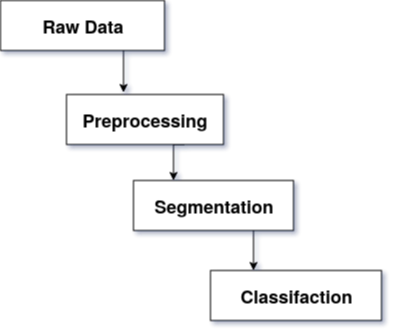
\includegraphics[scale = 0.52]{systemOverviw.png}
    \caption{System Overview}
    \label{fig:sysov}
\end{figure}{}
\section{DESIGN METHODOLOGY}



\section{CONCLUSION}



%%%%%%%%%%%%%%%%%%%%%%%%%%%%%%%%%%%%%%%%%%%%%%%%%%%%%%%%%%%%%%%%%%%%%%%%%%%%%%%
%
\section*{ACKNOWLEDGEMENT}



%%%%%%%%%%%%%%%%%%%%%%%%%%%%%%%%%%%%%%%%%%%%%%%%%%%%%%%%%%%%%%%%%%%%%%%%%%%%%%%
%
%\nocite{*}
\bibliographystyle{witseie}
\bibliography{sample}

%{\tiny \vfill \hfill \today \hspace{5mm} witseie-paper-2003.\TeX}

\end{document}

" vim: ts=4
" vim: tw=78
" vim: autoindent
" vim: shiftwidth=4
